\documentclass[11pt]{article}
\usepackage[letterpaper, margin=0.75in]{geometry}
\usepackage{graphicx}
\usepackage{xcolor}
\usepackage{hyperref}
\usepackage{fontspec}
\usepackage{wrapfig}

\definecolor{primarycolor}{HTML}{1a365d}
\definecolor{accentcolor}{HTML}{2b6cb0}
\definecolor{gray}{HTML}{718096}

\hypersetup{colorlinks=true, urlcolor=accentcolor}
\pagenumbering{gobble}
\setlength{\parindent}{0pt}

\begin{document}

% Logo in top-right corner
\begin{flushright}
    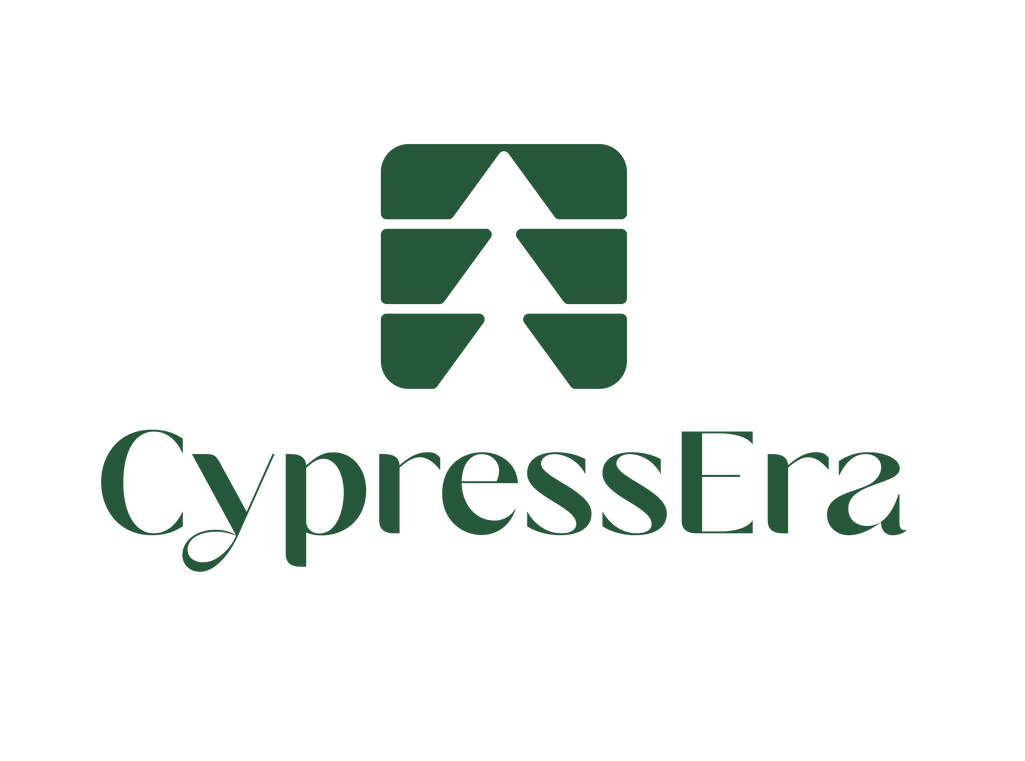
\includegraphics[height=0.8in]{logo.png}
\end{flushright}

\vspace{0.5em}

{\LARGE\color{primarycolor}\textbf{CypressEra AI Knowledge Base}}

\vspace{1.5em}

The AI Knowledge Base lets you upload your own documents---standards, manuals, project notes---so the AI assistant can reference them during analysis.

\section*{\color{primarycolor}Example}

Upload a document on NERC TPL-001 transmission planning standards, then ask:

\vspace{0.3em}
\begin{center}
    \textit{\color{accentcolor}``What are P6 contingencies?''}
\end{center}
\vspace{0.3em}

The AI retrieves relevant passages from your document and answers with source-backed accuracy.

\section*{\color{primarycolor}Getting Started}

Click ``+'' button and upload a PDF, DOCX, or TXT file.

\vfill

\begin{center}
    {\small\color{gray}\textcopyright\ CypressEra. All Rights Reserved.}
\end{center}

\end{document}
